

\documentclass[journal=jpcbfk]{achemso}

\usepackage[version=3]{mhchem}
\usepackage[T1]{fontenc}
\newcommand*\mycommand[1]{\texttt{\emph{#1}}}
\newcommand{\todo}[1]{\textcolor{red}{#1}}

\usepackage{rotating}
\usepackage{upgreek}				
\usepackage{xcolor}
\usepackage{booktabs}
\usepackage{multirow}
\usepackage{lmodern}
\usepackage{microtype}
\usepackage{xr}
\externaldocument{manuscript}
\usepackage{soul} % for highlights with \hl{} 



\author{Fernando Favela-Rosales}
\affiliation{Departamento de F\'isica, Centro de Investigaci\'on y de Estudios Avanzados del IPN, Apartado Postal 14-740, 07000 M\'exico D.F., M\'exico}

\author{Peter Heftberger}
%\email[]{samuli.ollila@aalto.fi}
%\homepage[]{Your web page}
%\thanks{}
%\altaffiliation{}
\affiliation{University of Graz}

\author{Matti Javanainen}
\affiliation{Department of Physics, Tampere University of Technology, Tampere, Finland}
\affiliation{University of Helsinki}

\author{Jesper J. Madsen}
\affiliation{Department of Global Health, College of Public Health}
\affiliation{University of South Florida}

\author{Josef Melcr}
\affiliation{Institute of Organic Chemistry and Biochemistry,
Academy of Sciences of the Czech Republic, 
Prague 6, Czech Republic}

\author{Markus Miettinen}
\affiliation{MPI}

\author{O. H. Samuli Ollila}
\email{samuli.ollila@helsinki.fi}
%\homepage[]{Your web page}
%\thanks{}
%\altaffiliation{}
\affiliation{Institute of Organic Chemistry and Biochemistry,
Academy of Sciences of the Czech Republic, 
Prague 6, Czech Republic}
\affiliation{Institute of Biotechnology, University of Helsinki}


\author{Georg Pabst}
\affiliation{University of Graz}

\author{Thomas Piggot}
\affiliation{University of Southampton}

% Collaboration name, if desired (requires use of superscriptaddress option in \documentclass). 
% \noaffiliation is required (may also be used with the \author command).
%\collaboration{}
%\noaffiliation


\SectionNumbersOn

\renewcommand{\thetable}{S\arabic{table}}%
\renewcommand{\thefigure}{S\arabic{figure}}%
\renewcommand{\thesection}{S\arabic{section}}%
\renewcommand{\thepage}{S\arabic{page}}%


\title{SUPPLEMENTARY INFORMATION: NMRlipids III: Lipid-cholesterol interactions in atomistic resolution molecular dynamics simulations} %Title of paper

\begin{document}

\section{CHARMM36 results from different simulation packages} \label{CHARMMprograms}
The results from CHARMM36 model for lipid bilayers from different 
simulation packages have been reported to give different results in
the literature \cite{piggot12,lee16}. The results are mainly
dependent on different Lennard-Jones cut-off settings, but
all the details are not quite understood. In this work we use
the results from Gromacs 5 with settings suggested to be optimal
by Gromacs webpage.~\todo{List these settings here or in SI.} We also compared the results from Gromacs 5 with
these settings to the results simulated with NAMD, OpenMM and literature
values. Based on comparison shown in Fig. \ref{programsCOMP}, we conclude
that Gromacs 5 with settings suggested in webpage gives consistent
results with the literature and other simulation packages. Thus these
results are used in the main body of the paper. However, order parameters
are slightly overestimated respected to the experiments also with these
settings. \\
\todo{Should be extend this discussion based on discussion at  https://github.com/NMRLipids/NmrLipidsCholXray/issues/4 ?}
 \begin{figure}[]
  \centering
  \includegraphics[width=8cm]{../FIGS/OrderParametersPROGRAMS.eps}

  \caption{\label{programsCOMP}
    Results for CHARMM36 model \cite{klauda10} from different simulation packages.
    Discussion going on at {\it https://github.com/NMRLipids/NmrLipidsCholXray/issues/4}.
  }
\end{figure}

\section{Order parameter slopes as a function of cholesterol}
 \begin{figure*}[]
  \centering
  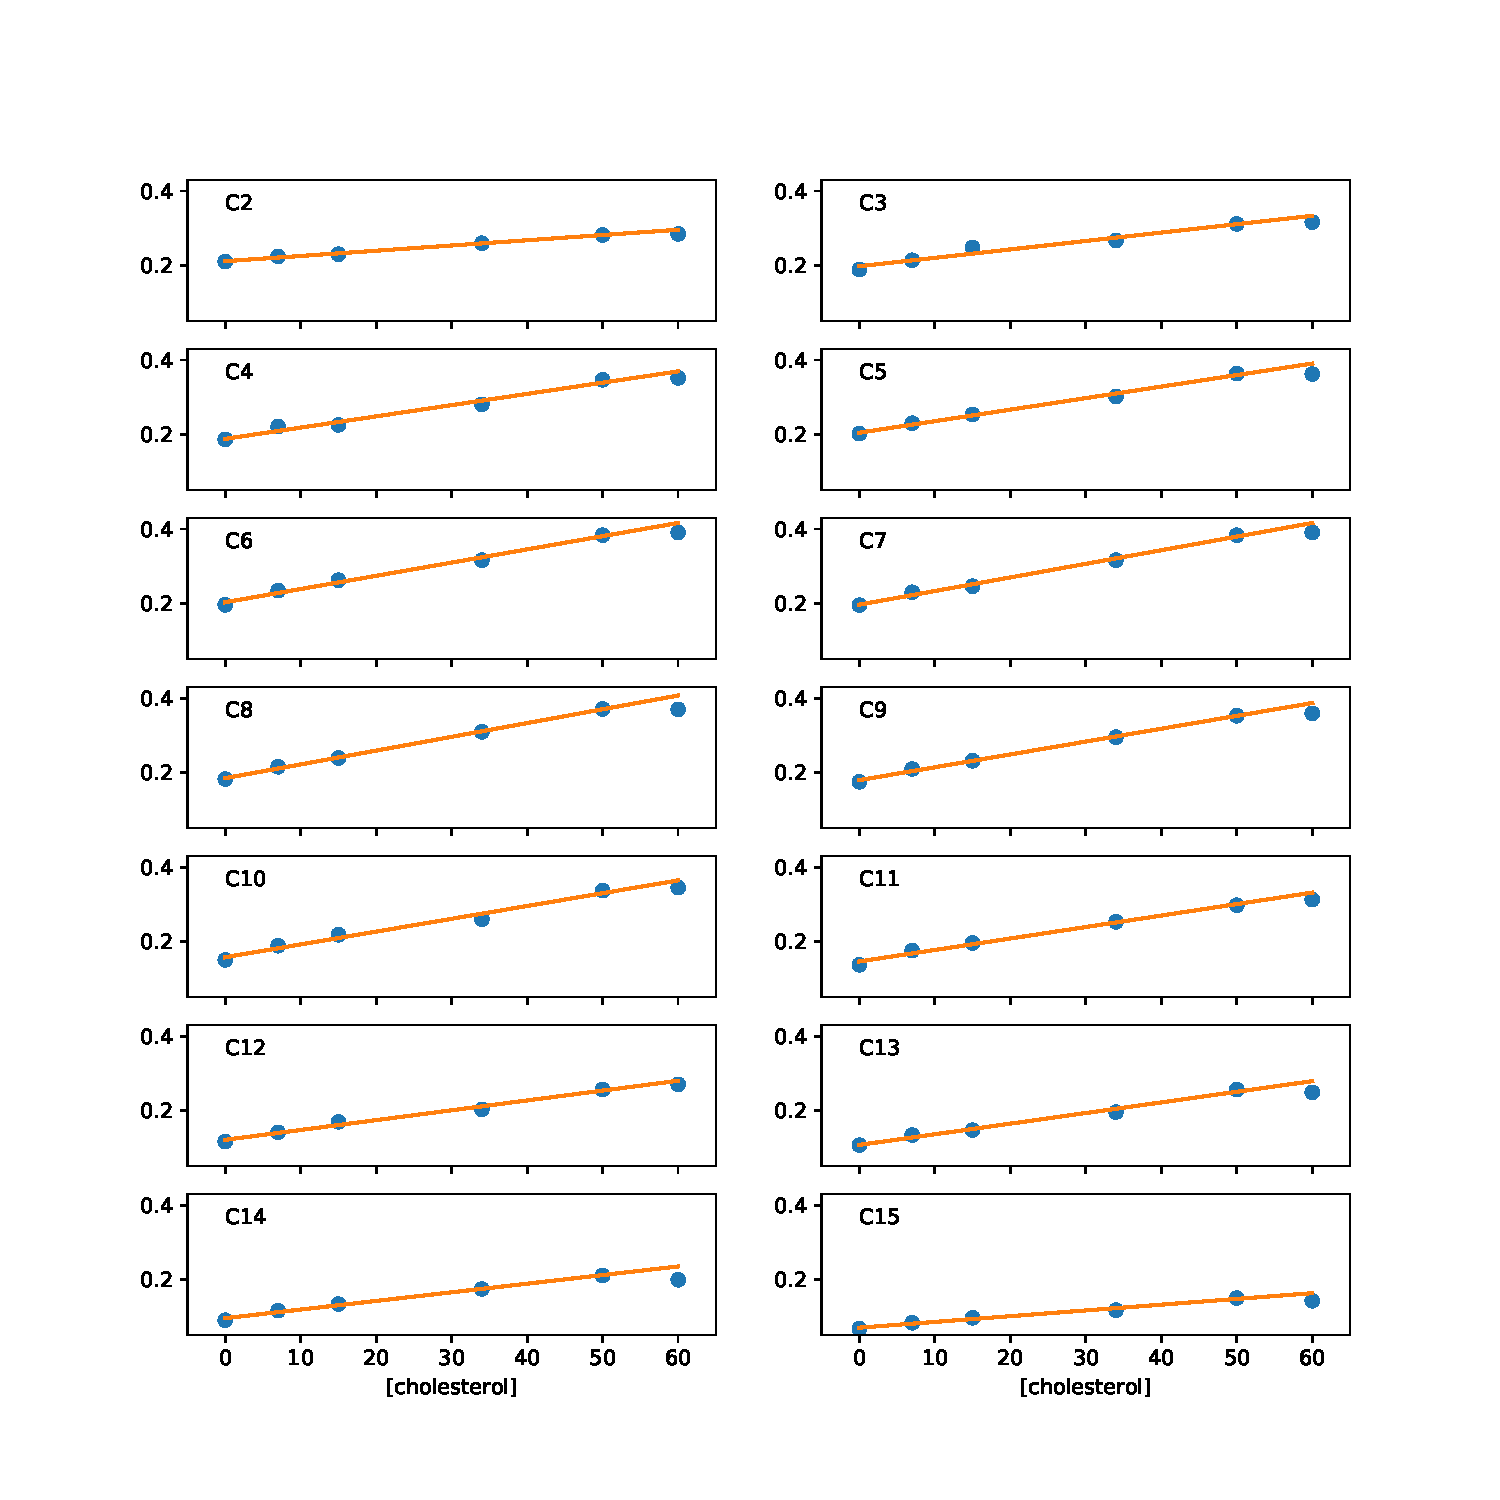
\includegraphics[width=19cm]{../FIGS/slopesEXPERIMENT.pdf}
  \caption{\label{slopes}
    Slopes of order parameters as a function of cholesterol from experiments \cite{ferreira13}.
  }
\end{figure*}

 \begin{figure*}[]
  \centering
  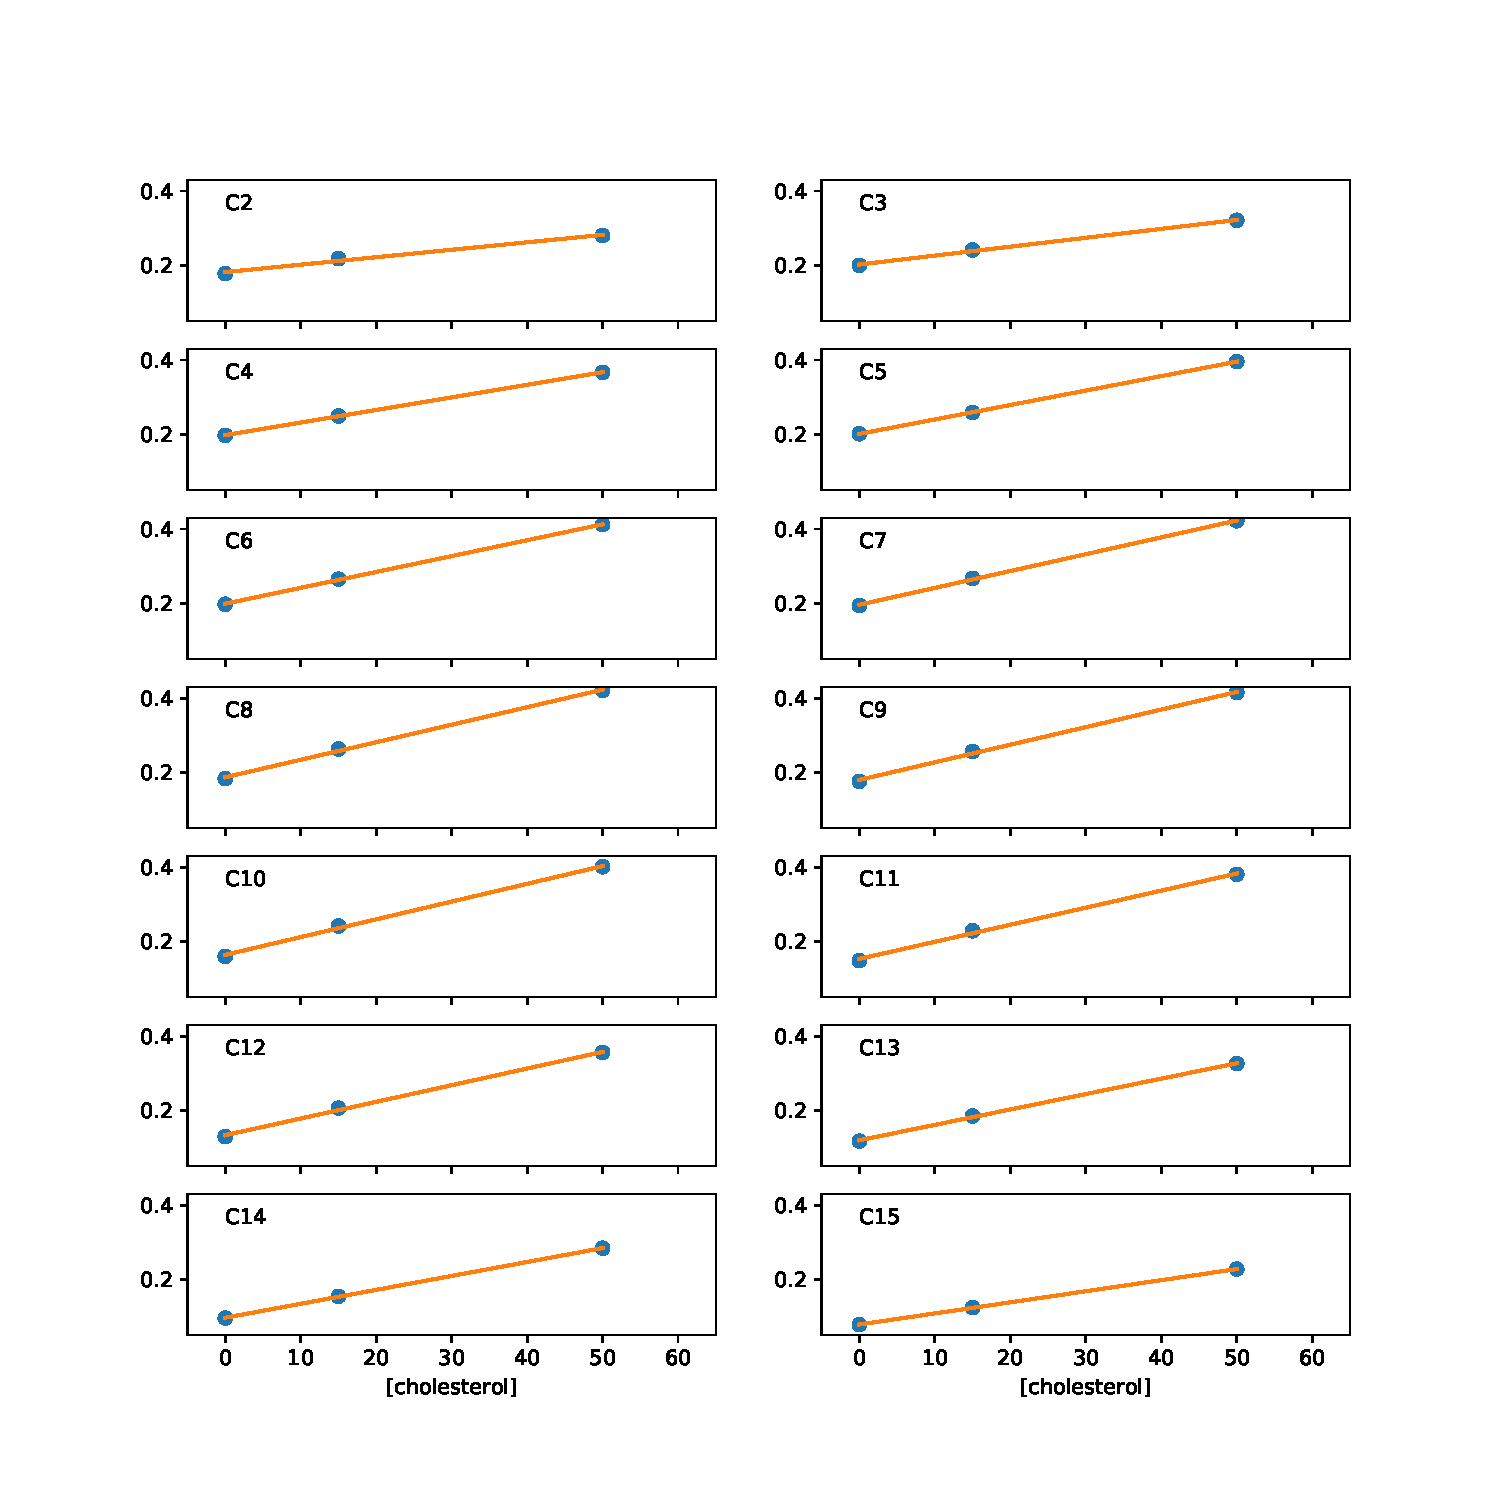
\includegraphics[width=19cm]{../FIGS/slopesBERGER.pdf}
  \caption{\label{slopesberger}
    Slopes of order parameters as a function of cholesterol from Berger simulations.
  }
\end{figure*}

 \begin{figure*}[]
  \centering
  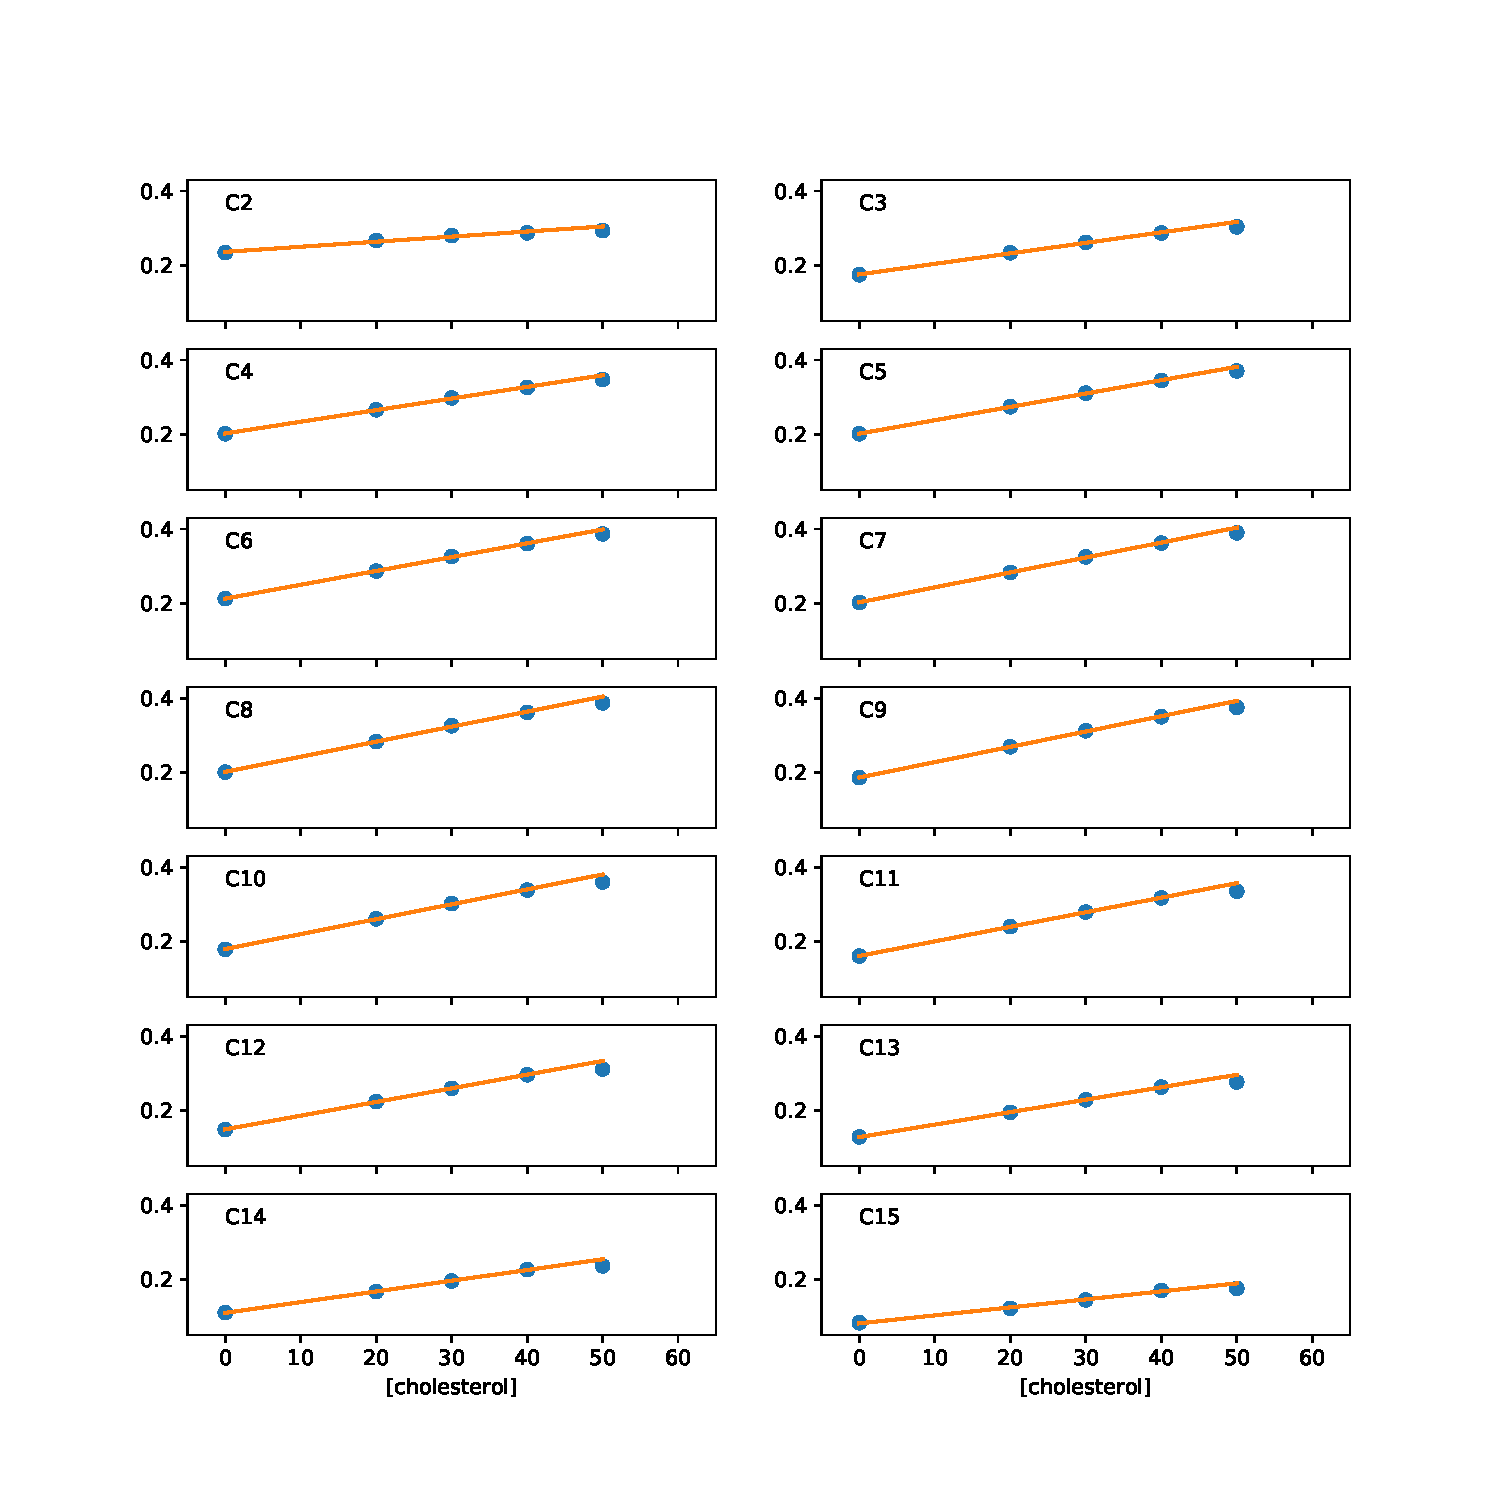
\includegraphics[width=19cm]{../FIGS/slopesCHARMM.pdf}
  \caption{\label{slopescharmm}
    Slopes of order parameters as a function of cholesterol from CHARMM36 simulations.
  }
\end{figure*}
 \begin{figure*}[]
  \centering
  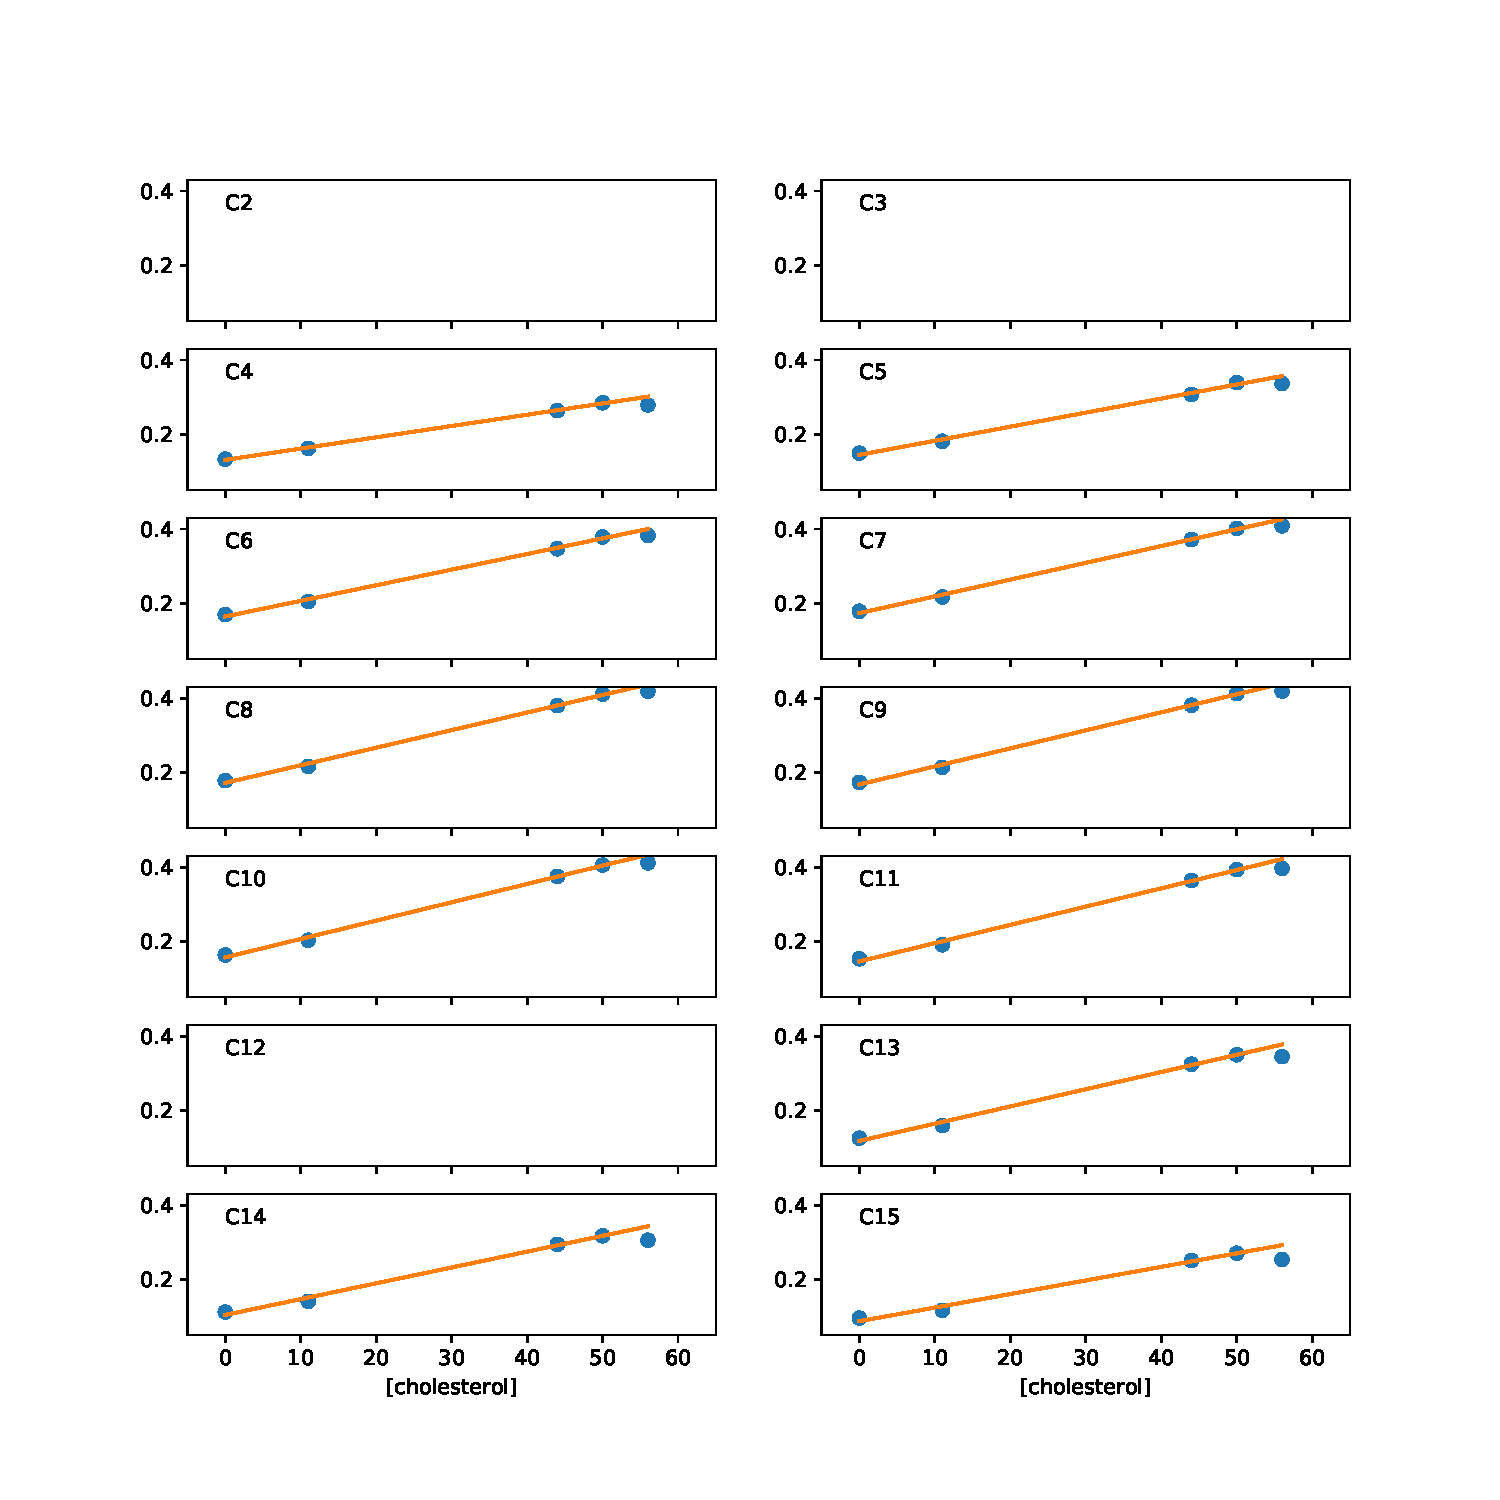
\includegraphics[width=19cm]{../FIGS/slopesMACROG.pdf}
  \caption{\label{slopesmacrog}
    Slopes of order parameters as a function of cholesterol from MacRog simulations.
  }
\end{figure*}
 \begin{figure*}[]
  \centering
  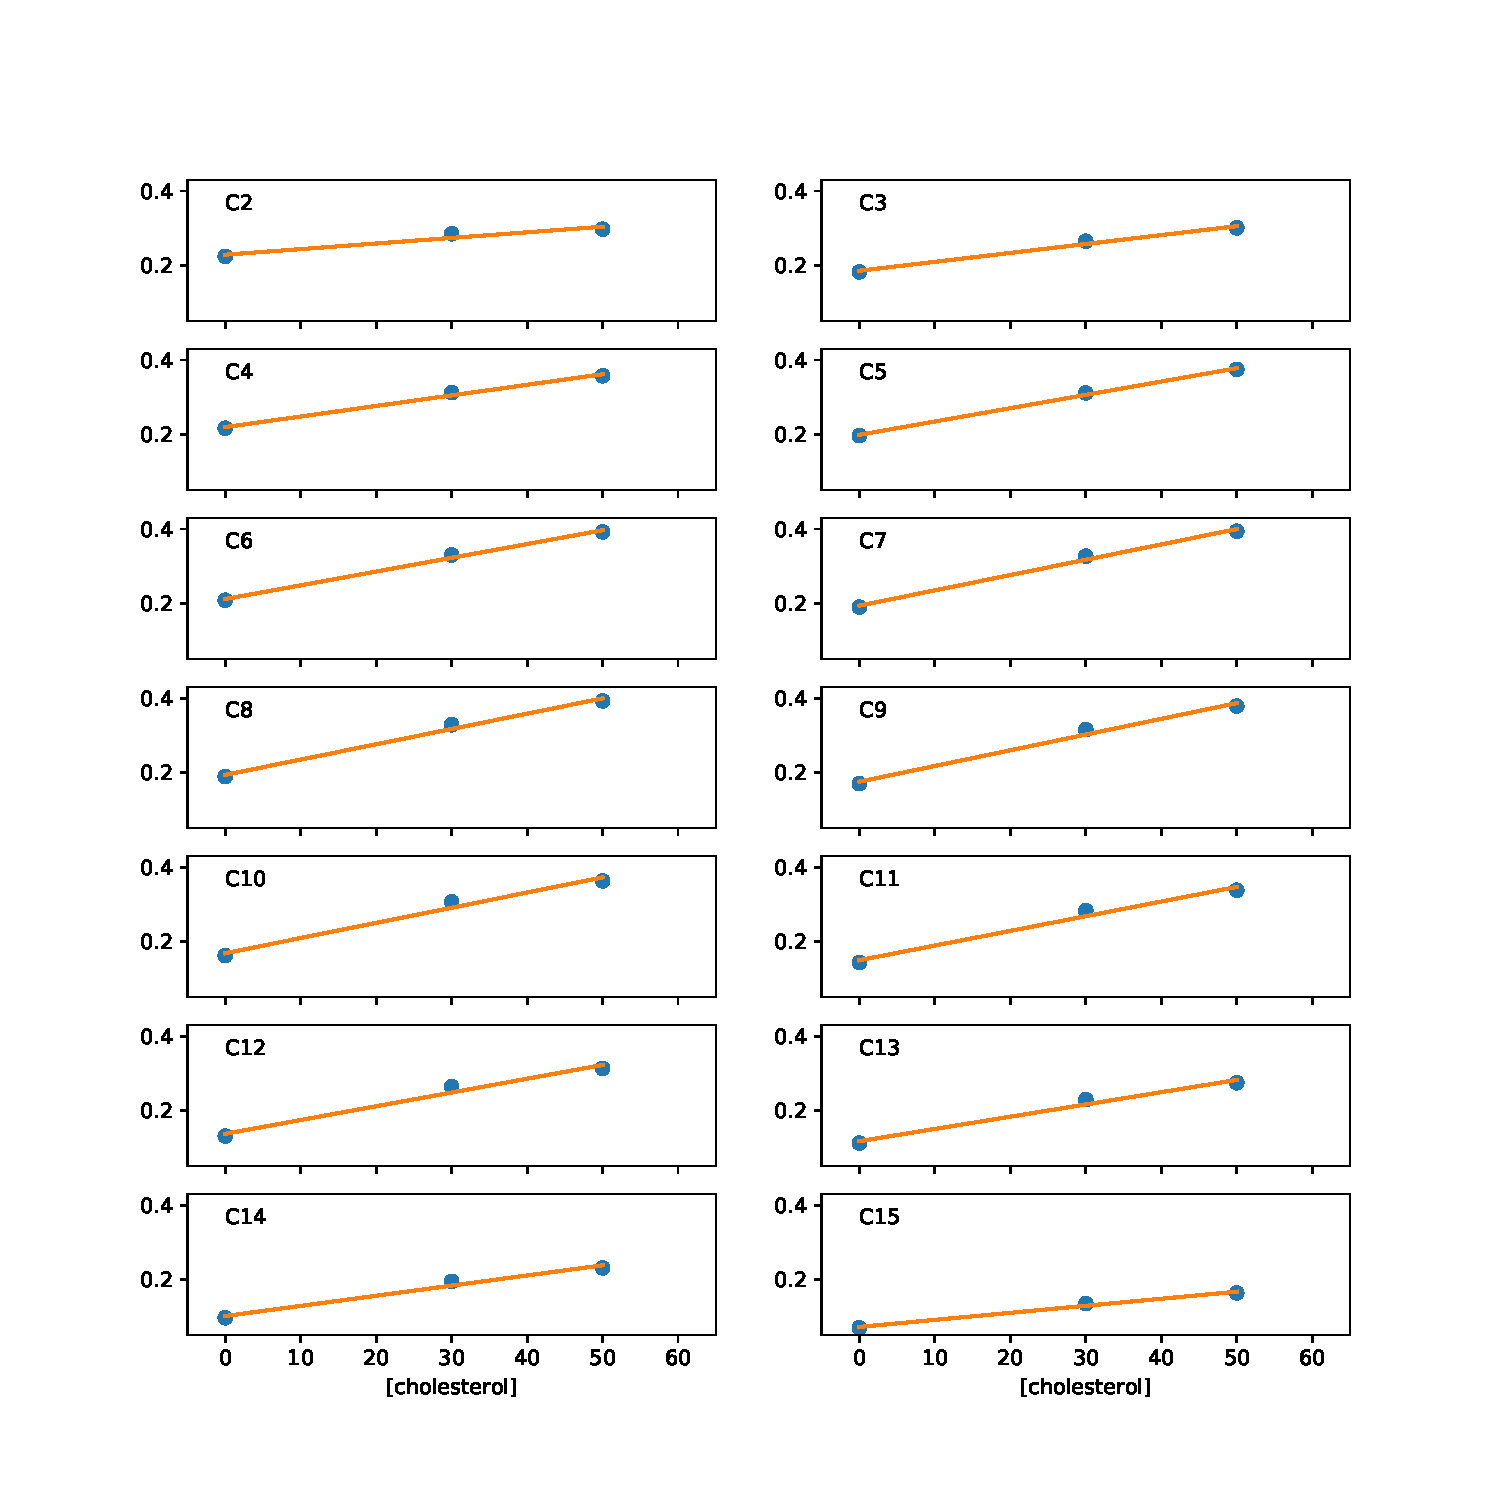
\includegraphics[width=19cm]{../FIGS/slopesSLIPIDS.pdf}
  \caption{\label{slopesslipids}
    Slopes of order parameters as a function of cholesterol from Slipids simulations.
  }
\end{figure*}
 \begin{figure*}[]
  \centering
  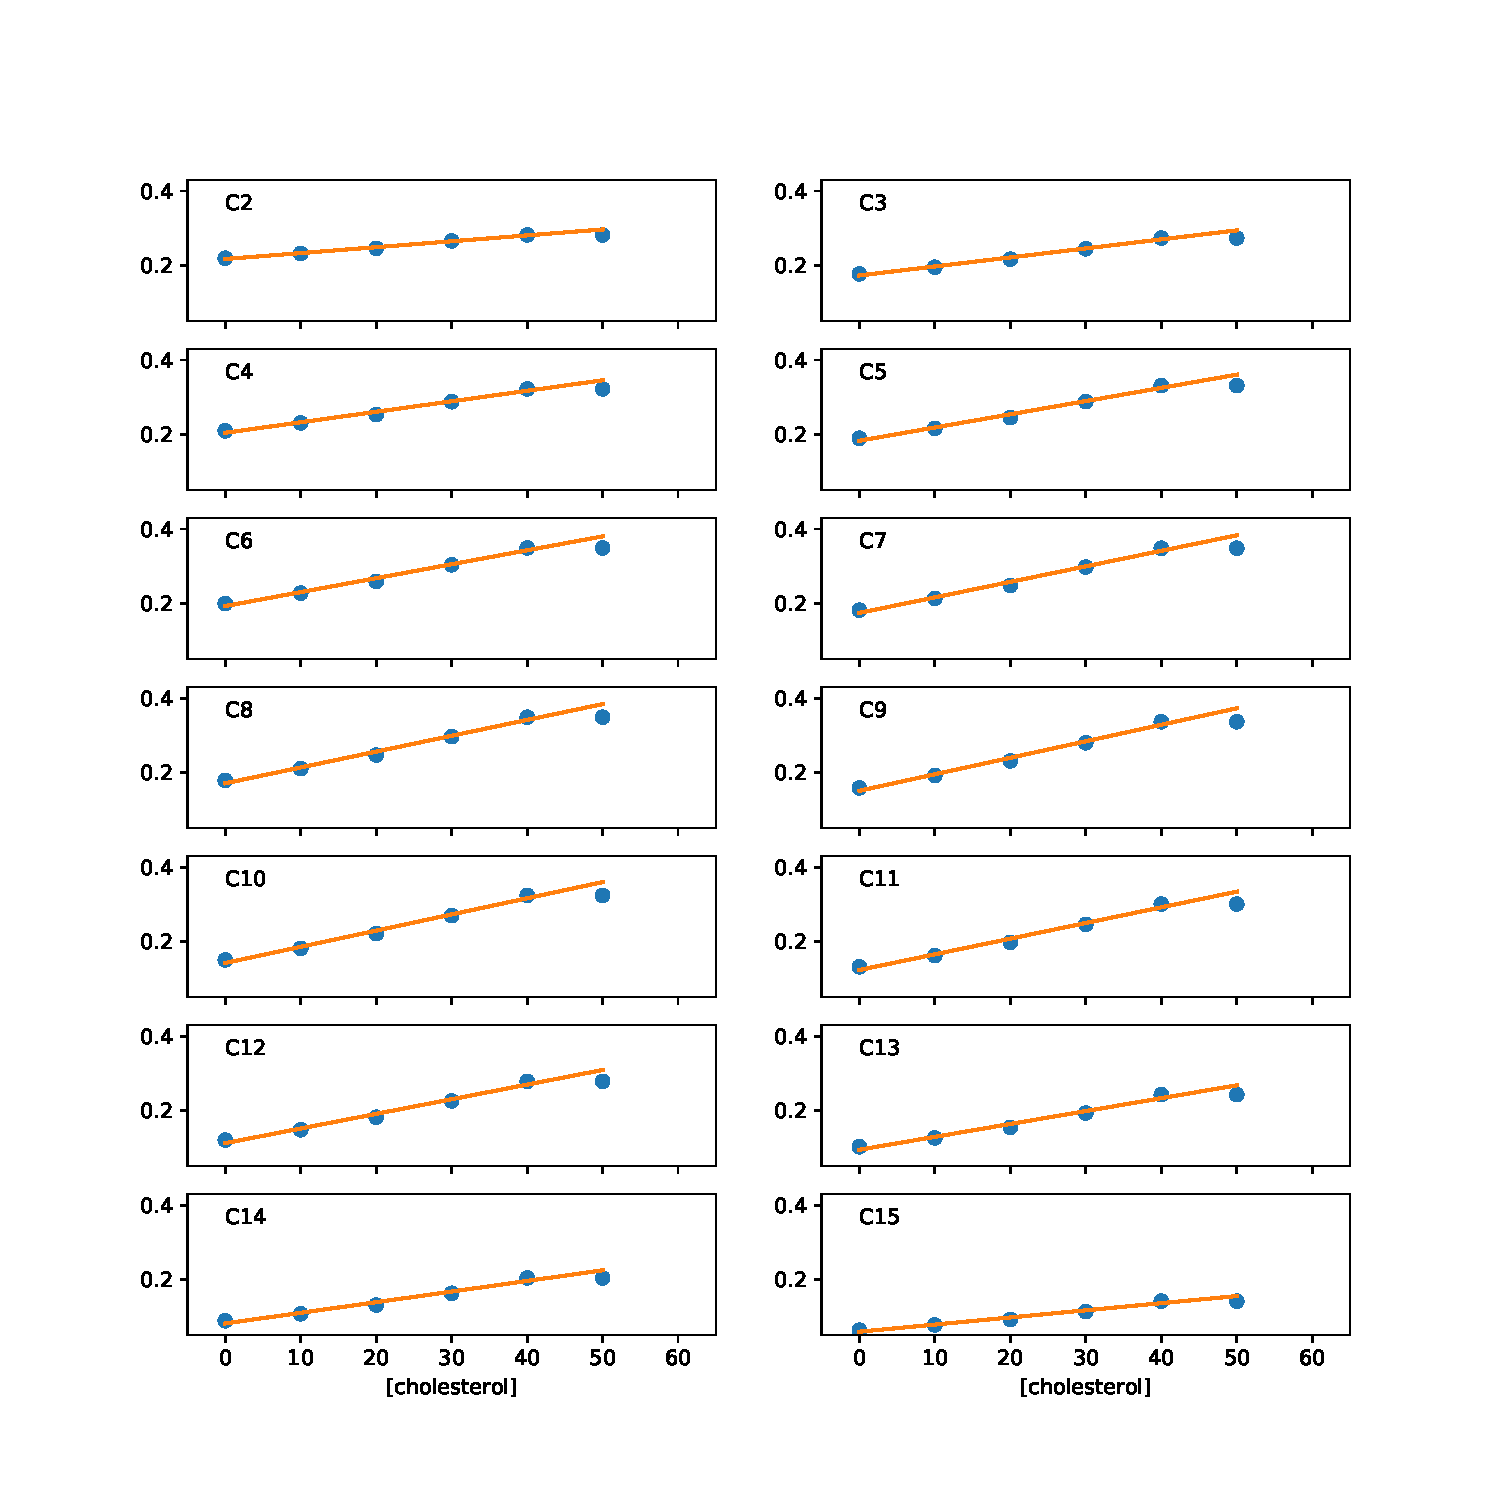
\includegraphics[width=19cm]{../FIGS/slopesSLIPIDST310K.pdf}
  \caption{\label{slopesslipids310K}
    Slopes of order parameters as a function of cholesterol from Slipids simulations at 298 K.
  }
\end{figure*}


 \section{Effect of undulations on order parameters} \label{undulations}
 \todo{This should be written based on contributions in this issue:
   https://github.com/NMRLipids/NmrLipidsCholXray/issues/16
 }
 
% \begin{figure}[]
%  \centering
%  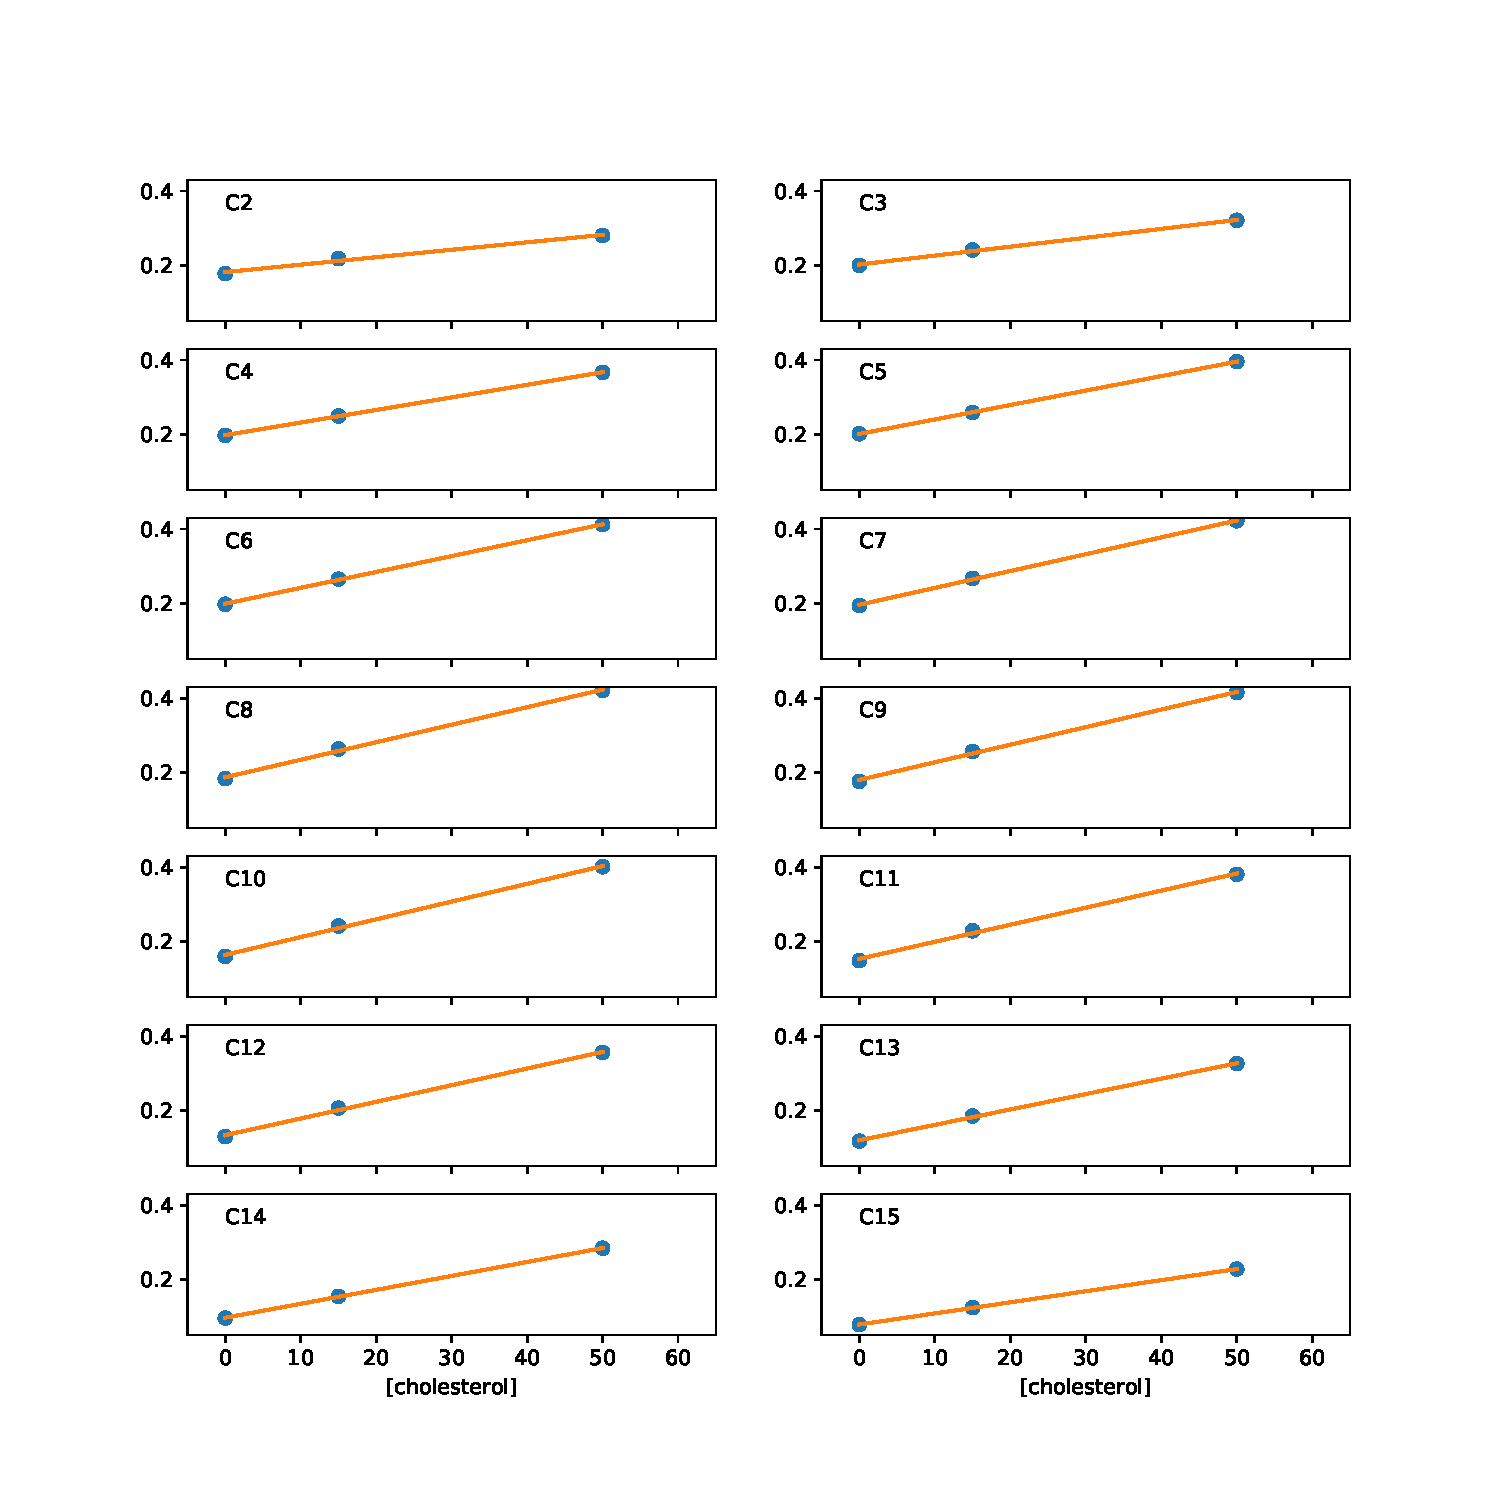
\includegraphics[width=8cm]{../FIGS/slopesBERGER.pdf}
%  \caption{\label{programsCOMP}
%    Slopes of order parameters as a function of cholesterol from Berger simulations.
%  }
%\end{figure}

% Create the reference section using BibTe
\bibliography{refs.bib}

%\newpage
%\section{APPENDIX: The NMR results reported by Tiago Ferreira}

%\listoftodos

\end{document}
%
% ****** End of file aiptemplate.tex ******
